\chapter{Forma canonică Jordan. Conice și cuadrice}

\section{Forma canonică Jordan}

După cum am văzut, nu orice matrice poate fi adusă la forma diagonală.
Însă vom vedea că, pentru spații vectoriale reale, orice matrice poate fi
adusă la \emph{forma canonică Jordan}, care este \qq{aproape diagonală},
într-un anume sens.

Prezentarea de mai jos urmează materialul \cite{brinz}, pp.\ 90--108.

Algoritmul va proceda similar cu cazul diagonalizării, în prima parte.

Fie $A \in M_n(\RR)$ o matrice căreia vrem să-i găsim forma canonică Jordan.
\begin{itemize}
\item Se calculează polinomul caracteristic al matricei, $ P_A(X) $, de unde
  se obțin valorile proprii, $ \sigma(A) = \{ \lambda_1, \dots, \lambda_p \} $;
\item Pentru fiecare valoare proprie, se determină vectorii proprii și subspațiile
  invariante corespunzătoare;
\item Pentru fiecare valoare proprie $ \lambda_i $, definim matricea
  $ M = A - \lambda_i I_n $. Observăm că $ \dr{Ker}M = V(\lambda_i) $.

  Pentru această matrice, se calculează \emph{șirul ascendent de nuclee}:
  \[
    V(\lambda_i) = \dr{Ker}M \subset \dr{Ker}M^2 \subset \dots \subset \dr{Ker}M^s,
  \]
  ultimul spațiu notîndu-se fie $ K(M) $, fie $ V^{\lambda_i} $ și numindu-se
  \emph{nucleu stabil} al lui $ M $.

  Prin definiție, $ \dim V^{\lambda_i} = m_a(\lambda_i) $.
\item Alegem vectori liniar independenți astfel:
  \begin{itemize}
  \item $ u_1, \dots, u_{p_1} \in \dr{Ker}M^s - \dr{Ker}M^{s - 1} $, astfel încît
    $ \dr{Ker}M^{s-1} \oplus \dr{Sp} \{ u_i \} \simeq \dr{Ker}M^s $. Altfel spus,
    completăm baza lui $ \dr{Ker}M^{s-1} $ la o bază a lui $ \dr{Ker}M^s $;
  \item Calculăm $ Mu_j^t \in \dr{Ker}M^{s-1} - \dr{Ker}M^{s-2} $ și
    completăm rezultatele la o bază a lui $ \dr{Ker}M^{s-1} $.
  \item Continuăm acești pași și în final se obține o listă de forma:
    \[
      \begin{cases}
        & u_1, \dots, u_{p_1} \\
        & Mu_1, \dots, Mu_{p_1}, u_{p_1 + 1}, \dots, u_{p_2} \\
        & \dots \\
        & M^{s-1}u_1, \dots, M^{s-1} up_1, \dots, u_{p_s}
      \end{cases}
    \]
    ultima linie reprezentînd o bază pentru $ V(\lambda_i) $, pe care o notăm
    cu $ B_1 $.
  \end{itemize}
\item Refacem pașii anteriori pentru fiecare valoare proprie și va rezulta
  $ B = B_1 \cup \dots\ cup B_p $ o bază a lui $ \RR^n $;
\item Fie $ T $ matricea de trecere de la baza canonică la această bază.
  Atunci forma canonică Jordan se scrie $ J = T^{-1} AT $.
\end{itemize}


\begin{remark}\label{rk:jordan-morf}
  Dacă, în loc de matrice, se pornește cu un endomorfism $ f $, se consideră
  mai întîi matricea asociată în baza canonică, $ A $, apoi putem continua
  ca mai sus.

  De asemenea, în locul matricei $ M $, putem gîndi că definim un nou
  endomorfism $ g = f - \lambda \dr{Id}_{\RR^n} $.
\end{remark}
%%%%%%%%%%%%%%%%%%%%%%%%%%%%%%%%%%%%%%%%%%%%%%%%%%%%%%%%%%%%%%%%%%%%%% 

\subsection{Exemple rezolvate}

Prezentăm în continuare cîteva exerciții rezolvate, în care insistăm
pe elementele de noutate. Am omis calculele intermediare, pe care le
puteți verifica ușor.

1. Fie matricea:
\[
  A = \begin{pmatrix}
    1 & -1 & -1 \\
    -3 & -4 & -3 \\
    4 & 7 & 6
  \end{pmatrix}.
\]

Calculăm forma canonică Jordan a acestei matrice.

Polinomul caracteristic este:
\[
  P_A(X) = \det(A - XI_3) = -(X + 1)(X - 2)^2,
\]
deci avem două valori proprii $ \lambda_1 = -1, m_a(-1) = 1 $ și
$ \lambda_2 = 2, m_a(2) = 2 $.

Fie $ \lambda_1 = -1 $. Definim $ M = A - \lambda_1 I_3 $.
Atunci $ \dr{Ker}M = V(\lambda_1) = \dr{Sp} \{(0, 1, -1)\} $. Deoarece
$ \dim V(\lambda_1) = 1 = m_g(\lambda_1) = m_a(\lambda_1) $, rezultă
că șirul nucleelor are un singur termen, deci lista va conține
doar $ u_1 = (0, 1, -1) $.

Fie acum $ \lambda_2 = 2 $. Definim $ M = A - \lambda_2 I_3 $.

Calculăm $ \dr{Ker}M = V(\lambda_2) = \dr{Sp} \{(1, 0, -1) \} $.
Cum $ m_a(\lambda_2) = 2 $, rezultă că șirul nucleelor va conține un pas și
va fi de forma $ V(\lambda_2) \subset V^{\lambda_2} $. Într-adevăr, calculăm:
\[
  V^{\lambda_2} = \dr{Ker}M^2 = \{ (x_1, x_2, x_3) \in \RR^3 \mid x_1 + 2x_2 + x_3 = 0 \}.
\]

Alegem $ u_2 \in V^{\lambda_2} - V(\lambda_2) $ astfel încît
$ V(\lambda_2) \oplus \dr{Sp} \{ u_2 \} = V^{\lambda_2} $. Altfel spus,
completăm baza lui $ V(\lambda_2) $ la o bază a lui $ V^{\lambda_2} $.

De exemplu, putem lua $ u_2 = (-2, 1, 0) $. Mai departe, calculăm $ Mu_2^t = (1, 0, -1) $.

Din lista $ \{ u_1, u_2, Mu_2^t \} $ obținem o bază a lui $ \RR^3 $, iar matricea
de trecere de la baza canonică va fi:
\[
  T = \begin{pmatrix}
    0 & -2 & 1 \\
    1 & 1 & 0 \\
    -1 & 0 & -1
  \end{pmatrix}
\]

Iar forma canonică Jordan este:
\[
  J = T^{-1}AT = \begin{pmatrix}
    -1 & 0 & 0 \\
    0 & 2 & 0 \\
    0 & 1 & 2
  \end{pmatrix}
\]

Spunem că această matrice este alcătuită din \emph{2 blocuri Jordan},
unul de mărime 2, asociat valorii proprii 2, iar unul de mărime 1,
asociat valorii proprii -1. Observați forma \qq{aproape diagonală} a matricei:
într-adevăr, blocul Jordan asociat valorii proprii 2 conține un element
nenul sub diagonală.

\vspace{1cm}

2. Fie matricea:
\[
  A = \begin{pmatrix}
    1 & 1 & 1 & 0 \\
    -1 & 3 & 0 & 1 \\
    -1 & 0 & -1 & 1 \\
    0 & -1 & -1 & 1
  \end{pmatrix}.
\]

Aducem această matrice la forma canonică Jordan.

Calculînd polinomul caracteristic, găsim:
\[
  P_A(X) = (X - 1)^4 \Rightarrow \sigma(A) = \{ 1 \}, m_a(1) = 4.
\]
Rezultă că $ V^\lambda \simeq \RR^4 $.

Calculăm spațiul vectorilor proprii și obținem:
\[
  V(\lambda) = \{ (\alpha, \beta, -\beta, \alpha - 2 \beta) \in \RR^4 \}.
\]
Definim $ M = A - \lambda I_4 $ și avem $ \dr{Ker}M = V(\lambda) $.

Cum $ m_g(\lambda) = 2 $, rezultă că șirul nucleelor va avea 3 termeni:
\[
  V(\lambda) = \dr{Ker} M \subset \dr{Ker}M^2 \subset V^\lambda \simeq \RR^4.
\]

Calculînd $ M^2 $ și apoi $ \dr{Ker}M^2 $, obținem:
\[
  \dr{Ker}M^2 = \{ (x_1, x_2, x_3, x_4) \in \RR^4 \mid x_1 - x_2 + x_3 - x_4 = 0 \},
\]
deci un spațiu de dimensiune 3.

Alegem $ u_1 \in V^\lambda - \dr{Ker}M^2 $ astfel încît
$ \dr{Ker}M^2 \oplus \dr{Sp} \{ u_1 \} = V^\lambda $.
Fie, de exemplu, $ u_1 = (1, 0, 0, 0) $.

Calculăm $ Mu_1^t = (0, -1, -1, 0) $ și $ M^2u_1^t = (-2, -2, 2, 2) $.

Acum alegem $ u_2 \in V(\lambda) $ astfel încît $ \{ M^2u_1^t, u_2 \} $ să
fie o bază a lui $ V(\lambda) $. Fie, de exemplu, $ u_2 = (1, 0, 0, 1) $.

Lista conține: $ u_1, Mu_1^t, M^2u_1, u_2 $, vectori independenți, suficienți
pentru o bază a lui $ \RR^4 $. Scriem matricea de trecere de la baza canonică:
\[
  T = \begin{pmatrix}
    1 & 0 & -2 & 1 \\
    0 & -1 & -2 & 0 \\
    0 & -1 & 2 & 0 \\
    0 & 0 & 2 & 1
  \end{pmatrix},
\]
iar forma Jordan se obține a fi:
\[
  J = T^{-1} AT = \begin{pmatrix}
    1 & 0 & 0 & 0 \\
    1 & 1 & 0 & 0 \\
    0 & 1 & 1 & 0 \\
    0 & 0 & 0 & 1
  \end{pmatrix}.
\]

Observăm că această matrice este alcătuită dintr-un bloc de mărime 3 și unul
de mărime 1, ambele corespunzătoare valorii proprii $ \lambda = 1 $.

%%%%%%%%%%%%%%%%%%%%%%%%%%%%%%%%%%%%%%%%%%%%%%%%%%%%%%%%%%%%%%%%%%%%%% 

\subsection{Exerciții propuse}


Aduceți la forma canonică Jordan endomorfismul:
\[
  f : \RR^3 \to \RR^3, \quad f(x, y, z) = (3x + y - z, 2y, x + y + z)
\]

și matricele:

\[
  A = \begin{pmatrix}
    4 & -1 & 1 \\
    1 & 3 & -1 \\
    0 & 1 & 1
  \end{pmatrix}, \quad
  B =
  \begin{pmatrix}
    1 & 1 & 1 & 0 \\
    -1 & 3 & 0 & 1 \\
    -1 & 0 & -1 & 1 \\
    0 & -1 & -1 & 1
  \end{pmatrix}, \quad
  C =
  \begin{pmatrix}
    0 & -1 & 0 \\
    -1 & -2 & 2 \\
    0 & -1 & 0
  \end{pmatrix}.
\]

%%%%%%%%%%%%%%%%%%%%%%%%%%%%%%%%%%%%%%%%%%%%%%%%%%%%%%%%%%%%%%%%%%%%%% 

\section{Conice}

Conicele sînt curbe plane, date de ecuații pătratice. Ele sînt reprezentate
în figura \ref{figure:conice}, împreună cu ecuațiile canonice.

\begin{figure}[!htbp]
  \centering
  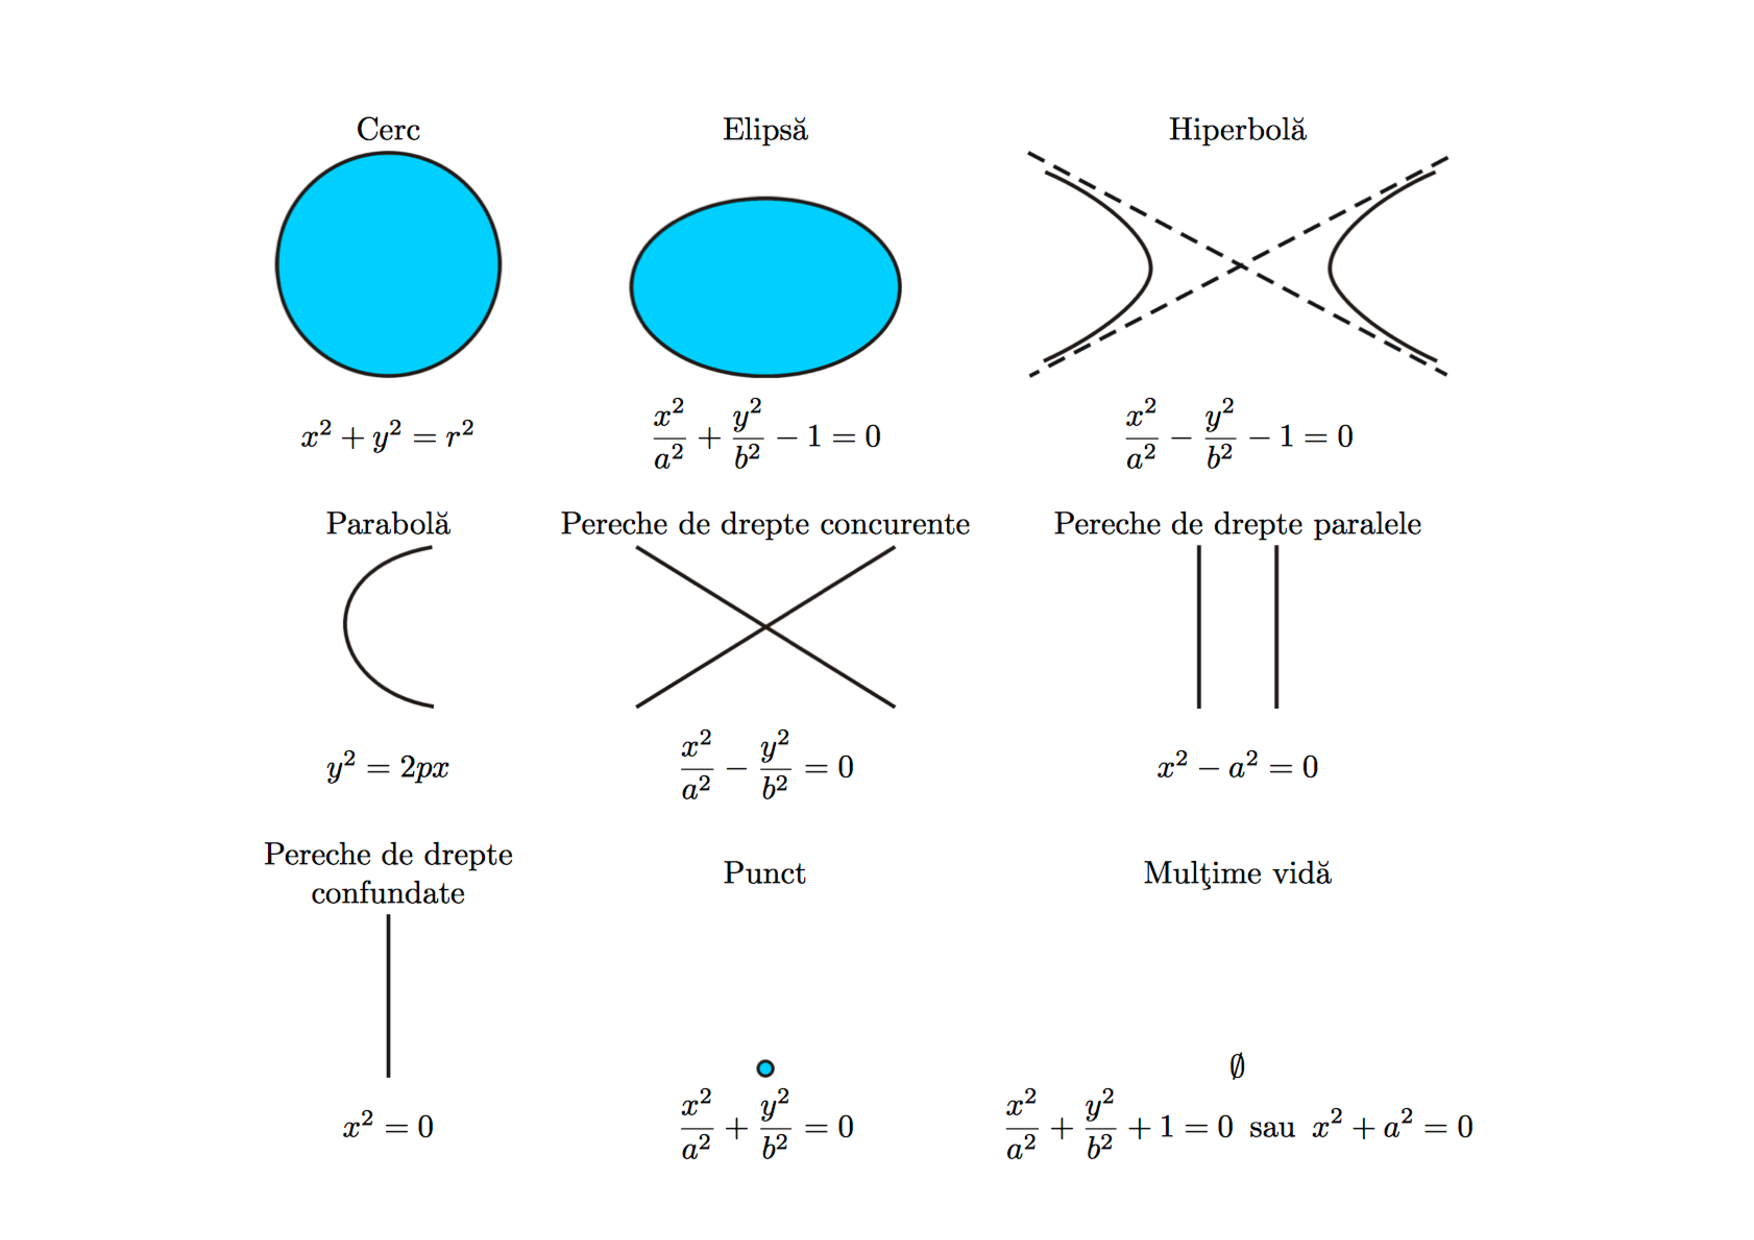
\includegraphics[scale = 0.5]{figs/conice}
  \caption{Conice și ecuațiile lor}
  \label{figure:conice}
\end{figure}

Scopul pe care ni-l propunem în această secțiune este să aducem o ecuație
a unei conice la forma canonică și să o reprezentăm grafic.

Vom prezenta algoritmul direct pe un exemplu. Metoda aplicată se
numește \emph{metoda rototranslației}, deoarece va folosi o operație
de rotație și una de translație a conicei.

Fie, de exemplu, conica:
\[
  g(x, y) = 3x^2 - 4xy - 2x + 4y - 3 = 0.
\]

Mai întîi, se scrie \emph{forma pătratică asociată}, adică alegem din conică
termenii de grad total 2:
\[
  q(x, y) = 3x^2 - 4xy.
\]

Apoi, scriem \emph{matricea asociată lui $q$}, care este:
\[
  A = \begin{pmatrix}
    3 & -2 \\
    -2 & 0
  \end{pmatrix}
\]

Această matrice se obține punînd coeficienții termenilor pătratici, în ordine
lexicografică. Dacă $ C(t) $ notează coeficientul termenului $ t $, atunci
matricea este, în forma generică:
\[
  A = \begin{pmatrix}
    C(x^2) & C(xy) \\
    C(yx) & C(y^2)
  \end{pmatrix},
\]
cu convenția că $ C(xy) = C(yx) $, deci în matrice vom avea jumătate din
coeficientul din forma pătratică.

Pentru această matrice, scriem ecuația caracteristică:
\[
  P_A(X) = \det(A - XI_2) = X^2 - 3X - 4 = (X + 1)(X - 4).
\]

Rezultă că valorile proprii sînt $ \sigma(A) = \{-1, 4 \} $.

În acest punct, putem face o observație de anticipație. Se numește
\emph{invariantul $ \delta $} al conicei produsul valorilor proprii.
Avem cazurile:
\begin{itemize}
\item $ \delta = \lambda_1 \cdot \lambda_2 > 0 \Rightarrow $ conica este elipsă;
\item $ \delta = \lambda_1 \cdot \lambda_2 < 0 \Rightarrow $ conica este hiperbolă;
\item $ \delta = \lambda_1 \cdot \lambda_2 = 0 \Rightarrow $ conica este parabolă.
\end{itemize}

În cazul nostru, vom obține o hiperbolă.

Mai departe, se calculează vectorii proprii și obținem:
\[
  V(\lambda_1) = \dr{Sp} \{(1, 2) \}, \quad V(\lambda_2) = \dr{Sp} \{(2, -1) \}.
\]

Vectorii din bazele subspațiilor proprii trebuie \emph{ortonormați} (de exemplu,
folosind procedura Gram-Schmidt). Observăm că ei sînt deja ortogonali, deci
mai trebuie doar să-i normăm:
\[
  ||(1, 2)|| = ||(2, -1)|| = \sqrt{5},
\]
deci obținem \emph{versorii proprii:}
\[
  e_1 = \Big(\frac{1}{\sqrt{5}}, \frac{2}{\sqrt{5}} \Big), \quad %
  e_2 = \Big(\frac{2}{\sqrt{5}}, \frac{-1}{\sqrt{5}} \Big)
\]

Acești versori vor alcătui coloanele \emph{matricei de rotație}:
\[
  R = \begin{pmatrix}
    \frac{1}{\sqrt{5}} & \frac{2}{\sqrt{5}} \\
    \frac{2}{\sqrt{5}} & \frac{-1}{\sqrt{5}}
  \end{pmatrix}
\]

În general, o matrice de rotație de unghi $ \theta $ (în sens trigonometric)
are forma:
\[
  R_\theta = \begin{pmatrix}
    \cos \theta & -\sin \theta \\
    \sin \theta & \cos \theta
  \end{pmatrix}
\]
și $ \det R_\theta = 1 $.

În cazul nostru, $ \det R = -1 $, deci putem schimba între ele coloanele
și obținem o matrice de rotație (echivalent, putem schimba orientarea unuia
dintre versori, de exemplu, $ e_1 \longrightarrow -e_1 $).

Apoi aplicăm rotația, adică, dacă $ (x, y) $ sînt vechile coordonate,
coordonatele din sistemul rotit $ (x', y') $ se obțin din ecuația:
\[
  \begin{pmatrix}
    x \\ y
  \end{pmatrix} = R \cdot \begin{pmatrix} x_1 \\ y_1 \end{pmatrix}
\]

Cu alte cuvinte, avem sistemul:
\[
  \begin{cases}
    x &= \frac{-1}{\sqrt{5}} x_ + \frac{2}{\sqrt{5}} y_1 \\
    y &= \frac{-2}{\sqrt{5}} x_1 + \frac{-1}{\sqrt{5}} y_1
  \end{cases}.
\]

Aceste coordonate se înlocuiesc în ecuația inițială a conicei și obținem
\emph{conica rotită}:
\[
  -x_1^2 + 4y_1^2 - \frac{6}{\sqrt{5}} x_1 - \frac{8}{\sqrt{5}} y_1 - 3 = 0.
\]

Prelucrăm algebric, completînd pătratele, și obținem:
\[
  -\Big( x_1 + \frac{3}{\sqrt{5}} \Big)^2 + 4 \Big(y_1 - \frac{1}{\sqrt{5}} \Big)^2 = 2.
\]

Facem acum \emph{translația}:
\[
  \begin{cases}
    X &= x_1 + \frac{3}{\sqrt{5}} \\
    Y &= y_1 - \frac{1}{\sqrt{5}}
  \end{cases}
\]
și obținem:
\[
  -X^2 + 4Y^2 = 2 \Leftrightarrow %
  -\Big( \frac{X}{\sqrt{2}} \Big)^2 + \Big( \frac{Y}{1/2} \Big)^2 = 1,
\]
deci ecuația unei hiperbole.

Pentru reprezentarea grafică, trebuie să ținem cont de operațiile efectuate:
\begin{itemize}
\item rotația de unghi $ \theta $, cu proprietatea că $ \cos \theta = -\dfrac{1}{\sqrt{5}} $,
  deci $ \theta \simeq \dfrac{2\pi}{3} $;
\item translația centrului cu $ \dfrac{3}{\sqrt{5}} $ pe axa $ OX $ și
  $ -\dfrac{1}{\sqrt{5}} $ pe axa $ OY $.
\end{itemize}

Mai putem determina și \emph{centrul conicei}, din sistemul:
\[
  \begin{cases}
    \dfrac{\partial g}{\partial x} &= 0 \\
    & \\    
    \dfrac{\partial g}{\partial y} &= 0
  \end{cases}
\]

Soluția sistemului este centrul conicei, de coordonate $ C(1, 1) $.

Reprezentarea grafică (folosind \href{https://www.geogebra.org/}{GeoGebra}) este
redată în figura \ref{fig:hiperbola-geog}.

\begin{figure}[!htbp]
  \centering
  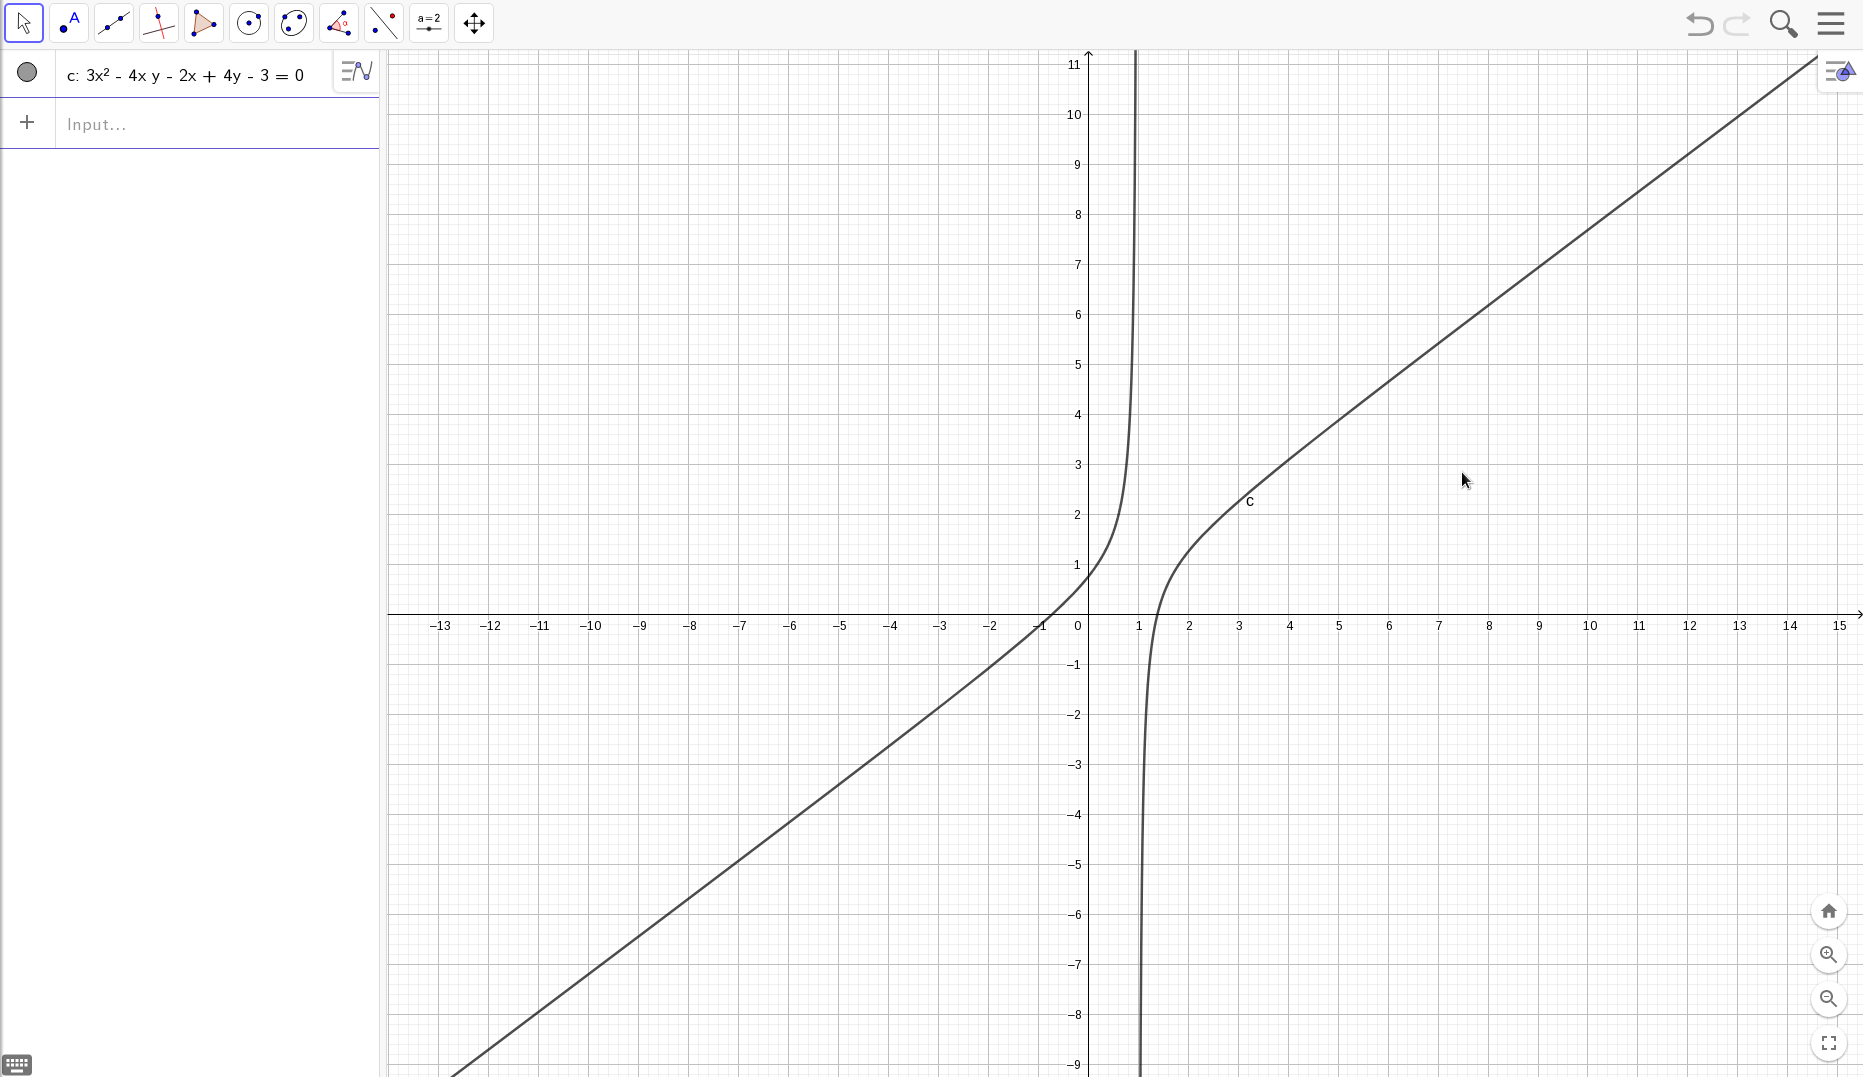
\includegraphics[scale = 0.3]{figs/hiperbola-geogebra.png}
  \caption{Hiperbola $3x^2 - 4xy - 2x + 4y - 3 = 0$}
  \label{fig:hiperbola-geog}
\end{figure}

%%%%%%%%%%%%%%%%%%%%%%%%%%%%%%%%%%%%%%%%%%%%%%%%%%%%%%%%%%%%%%%%%%%%%% 

\section{Cuadrice}

Cuadricele sînt suprafețe care pot fi obținute prin rotirea unei conice în jurul
unei axe. Astfel, din elipsă, de exemplu, obținem elipsoizi, din parabolă,
paraboloizi, iar din hiperbolă, hiperboloizi.

Formele, împreună cu ecuațiile canonice, pot fi consultate, de exemplu,
\href{https://en.wikipedia.org/wiki/Quadric#Euclidean_space}{aici}.

Procedura de a aduce o cuadrică la forma canonică funcționează ca în cazul
conicelor.

Mai jos un exemplu rezolvat.

\[
  x^2 + 3y^2 + 4yz - 6x + 8y + 8 = 0.
\]

Considerăm forma pătratică asociată:
\[
  g = x^2 + 3y^2 + 4yz,
\]
care are matricea simetrică.
\[
  A = \begin{pmatrix}
    1 & 0 & 0 \\
    0 & 3 & 2 \\
    0 & 2 & 0
  \end{pmatrix}
\]
Ecuația caracteristică rezultă: $(1 - \lambda)(\lambda^2 - 3\lambda - 4) = 0$,
deci $\lambda_1 = 1, \lambda_2 = -1, \lambda_3 = 4$.

Găsim subspațiile invariante:
\begin{align*}
  V(\lambda_1) &= \Bigg\{ (x, y, z) \in \RR^3 \mid %
                 \begin{pmatrix}
                   0 & 0 & 0 \\
                   0 & 2 & 2 \\
                   0 & 2 & -1
                 \end{pmatrix} \cdot
                           \begin{pmatrix}
                             x \\ y \\ z
                           \end{pmatrix}  =
  \begin{pmatrix}
    0 \\ 0 \\ 0
  \end{pmatrix} \Bigg\} \\
               &= \{ (x, 0, 0) \mid x \in \RR \}
\end{align*}

Similar:
\begin{align*}
  V(\lambda_2) &= \{ (0, y, -2y) \mid y \in \RR \} \\
  V(\lambda_3) &= \{ (0, 2z, z) \mid z \in \RR \}.
\end{align*}

Alegem vectori proprii ortonormați particularizînd elemente din
subspațiile invariante.
De exemplu:
\[
  e_1 = (1, 0, 0), \quad e_2 = \frac{1}{\sqrt{5}} (0, 1, -2), %
  \quad e_3 = \frac{1}{\sqrt{5}}(0, 2, 1).
\]
Matricea $R$ cu acești vectori pe coloane are proprietatea $\det R = 1$, deci
este o matrice de rotație. O aplicăm și găsim schimbarea de coordonate:
\[
  \begin{cases}
    x &= x' \\
    y &= \frac{1}{\sqrt{5}} (y' + 2z') \\
    z &= \frac{1}{\sqrt{5}} (-2y' + z')
  \end{cases}
\]

Ecuația cuadricei devine:
\[
  x^{\prime 2} - y^{\prime 2} + 4 z^{\prime 2} - 6x^\prime + %
  \frac{8}{\sqrt{5}} y^\prime + \frac{16}{\sqrt{5}} z^\prime + 8 = 0.
\]

Formăm pătrate și obținem:
\[
  (x' - 3)^2 - \big( y' - \frac{4}{\sqrt{5}} \big)^2 + %
  4 \big(z' + \frac{2}{\sqrt{5}} \big)^2 - 1 = 0.
\]

Efectuăm translația corespunzătoare noilor coordonate și obținem:
\[
  X^2 - Y^2 + 4Z^2 - 1 = 0 \Leftrightarrow X^2 - Y^2 + \frac{Z^2}{\frac{1}{4}} - 1 = 0,
\]
adică un hiperboloid cu o pînză.

%%%%%%%%%%%%%%%%%%%%%%%%%%%%%%%%%%%%%%%%%%%%%%%%%%%%%%%%%%%%%%%%%%%%%%

\section{Exerciții propuse}

1. Aduceți următoarele conice la forma canonică și reprezentați-le:
\begin{enumerate}[(a)]
\item $ 4xy - 3y^2 + 4x - 14y - 7 = 0 $ (hiperbolă);
\item $ 9x^2 - 6xy + y^2 + 20x = 0 $ (parabolă);
\item $ x^2 - 2xy + 3y^2 - 4x + 6y - 4 = 0 $ (elipsă);
\item $ 5x^2 + 8xy + 5y^2 - 18x - 18y + 9 = 0 $ (elipsă);
\item $ x^2 - 4xy + 4y^2 - 6x + 2y + 1 = 0 $ (parabolă)
\end{enumerate}

\vspace{1cm}

2. Aceeași cerință pentru cuadrica:
\[
  x^2 - y^2 + z^2 - 2xy - 2yz - 2zx - 5x - 1 = 0
\]
(hiperboloid cu o pînză).


%%% Local Variables:
%%% mode: latex
%%% TeX-master: "../ag-18-19"
%%% End:
